\thispagestyle{empty}
\subsection{Queue}
\subsubsection*{Recursion Queue (Array version)}
\begin{itemize}
	\item \textbf{Theoretical Time Complexity:} Both implementations have the same theoretical time complexity of O(1) for \verb|enqueue| and O(n) for \verb|copy| operations.
	\item \textbf{Practical Performance:}
	      \begin{itemize}
		      \item  Loop-based implementations are generally faster in practice because they avoid the overhead of function calls and recursion.
		      \item The recursive version doesn't work well with large data sets because of stack overflow.
	      \end{itemize}
\end{itemize}
\begin{figure}[!ht]
	\centering
	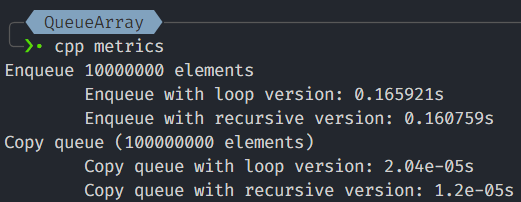
\includegraphics[width=0.6\textwidth]{imgs/QueueArray/metrics.png}
	\caption{Recursive and loop version comparison of Queue (Array version)}\label{fig:queue_arr_metrics}
\end{figure}

\subsubsection*{Recursion Queue (Linked List version)}
\begin{itemize}
	\item \textbf{Theoretical Time Complexity:} Both implementations have the same theoretical time complexity of O(1) for \verb|enqueue| and O(n) for  \verb|release| operations.
	\item \textbf{Practical Performance:}
	      \begin{itemize}
		      \item  Loop-based implementations are generally faster in practice because they avoid the overhead of function calls and recursion.
		      \item The recursive version doesn't work well with large data sets because of stack overflow.
	      \end{itemize}
\end{itemize}
\begin{figure}[!ht]
	\centering
	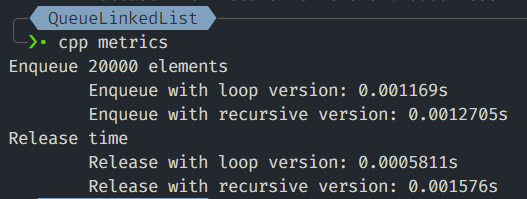
\includegraphics[width=0.6\textwidth]{imgs/QueueLinkedList/metrics.png}
	\caption{Recursive and loop version comparison of Queue (Linked List version)}\label{fig:queue_ll_metrics}
\end{figure}